\documentclass[12pt, titlepage]{article}
\usepackage{beamerarticle}
\usepackage[utf8]{inputenc}
\usepackage{hyperref}
\usepackage{amssymb,amsmath}

% Page settings
\usepackage[letterpaper, margin=1in]{geometry}
\usepackage{times}
%\usepackage{palatino}%\usepackage{lmodern, times}
%\usepackage{lmodern}%\usepackage{lmodern, times}
\usepackage{setspace}                           
\onehalfspacing %\doublespacing  % \singlespacing 

% Appendix
\usepackage{appendix}

% Line numbers
%\usepackage{lineno}
%\linenumbers


% Tables
\usepackage{array,booktabs,longtable,rotating}
\newenvironment{tablenotes}[1][]{
  \begin{minipage}{\textwidth}\emph{Notes:}{\footnotesize #1}
}{\end{minipage}}
\makeatletter
\def\fps@table{htbp}
\makeatother

% Graphics
\usepackage{graphicx,grffile}
\makeatletter
\def\maxwidth{\ifdim\Gin@nat@width>\linewidth\linewidth\else\Gin@nat@width\fi}
\def\maxheight{\ifdim\Gin@nat@height>\textheight\textheight\else\Gin@nat@height\fi}
\makeatother
% Scale images if necessary, so that they will not overflow the page
% margins by default, and it is still possible to overwrite the defaults
% using explicit options in \includegraphics[width, height, ...]{}
\setkeys{Gin}{width=\maxwidth,height=\maxheight,keepaspectratio}
% set default figure placement to htbp
\makeatletter
\def\fps@figure{htbp}
\makeatother

\usepackage{natbib}% plainnat
\bibliographystyle{abbrvnat}
\setcitestyle{authoryear,open={(},close={)}}
%\bibliographystyle{aer}


\setlength{\emergencystretch}{3em}  % prevent overfull lines
\providecommand{\tightlist}{%
  \setlength{\itemsep}{0pt}\setlength{\parskip}{0pt}}



\institute{}
\titlegraphic{}

\usepackage{xcolor}
\newcommand\todonote[1]{\textcolor{red}{#1}}



% Subscript
\newcommand\sub[1]{_{#1}}
\newcommand\supsc[1]{^{#1}}

\title{Gender Imbalance Online\thanks{Blasco: Harvard Institute for Quantitative Social Science, Harvard
University, 1737 Cambridge Street, Cambridge, MA 02138 (email:
\href{mailto:ablasco@fas.harvard.edu}{\nolinkurl{ablasco@fas.harvard.edu}}).
Lakhani: Harvard Business School, Soldiers Field, Boston, MA 02163, and
National Bureau of Economic Research (email:
\href{mailto:k@hbs.edu}{\nolinkurl{k@hbs.edu}}). Menietti: Harvard
Institute for Quantitative Social Science, Harvard University, 1737
Cambridge Street, Cambridge, MA 02138 (email:
\href{mailto:mmenietti@fas.harvard.edu}{\nolinkurl{mmenietti@fas.harvard.edu}}).
We gratefully acknowledge the financial support of XXXX.}}
\author{Andrea Blasco \and Karim R. Lakhani \and Michael Menietti}
\date{Last updated: 13 April, 2017}

\begin{document}
\maketitle
\begin{abstract}
We report results of a natural field experiment conducted XXXX.

\smallskip\noindent 
JEL Classification: XXXX.

\smallskip\noindent 
Keywords: XXXX.
\end{abstract}


% Todo notes
%\usepackage[textsize=tiny]{todonotes}
%\newcommand\redmarginpar[1]{\marginpar{\footnotesize{\textcolor{red}{#1}}}}
%\listoftodos[Notes]
\clearpage

\section{Introduction}\label{introduction}

Though the proportion of Internet users is nearly the same across the
genders, researchers have found significant gender imbalances in online
behavior:

\begin{itemize}
\tightlist
\item
  Only 13 percent of Wikipedia contributors are women
  \citep{hill2013wikipedia};
\item
  Wikipedia articles on women are more likely to be missing than are
  articles on men relative to Britannica \citep{reagle2011gender};
\item
  Less than 5 percent of StackOverflow users answering technical
  questions are women \citep{vasilescu2012gender};
\item
  Women make a small fraction of people going to hackathons or taking
  part in online competitions on crowdsourcing platforms (Innocentive,
  TopCoder, Kaggle).
\end{itemize}

The reasons behind this gender gap are not fully understood. It is clear
that it is not due to discriminatory rules put in place on these
platforms. Rather the culprit seems to be a mix of psychological
motivations and institutional characteristics of the platforms that
might have inadvertently promoted an imbalance.

We conjecture that an important mechanism of imbalance could be the
combination of

\begin{enumerate}
\def\labelenumi{\arabic{enumi}.}
\tightlist
\item
  Gamification \& incentives
\item
  Differences in preferences between the genders
\end{enumerate}

Online platforms use elements of game play to engage their members
(rankings, game points, competition with others, etc.) and stimulate
higher levels of user activity. If men and women have different
inclinations towards these incentives, they might inadvertently
stimulate an imbalanced participation.

\section{Experimental design}\label{experimental-design}

\subsection{Profiles selection}\label{profiles-selection}

\begin{enumerate}
\def\labelenumi{\arabic{enumi}.}
\tightlist
\item
  Recruitment profiles\ldots{}
\item
  Consent profiles\ldots{}
\item
  Profile survey\ldots{}
\end{enumerate}

Evaluation at CLER

\begin{enumerate}
\def\labelenumi{\arabic{enumi}.}
\tightlist
\item
  Recruitment\ldots{}
\item
  Consent for CLER\ldots{}
\end{enumerate}

\subsection{Preliminary/final survey}\label{preliminaryfinal-survey}

\begin{enumerate}
\def\labelenumi{\arabic{enumi}.}
\tightlist
\item
  Recruit survey\ldots{}
\item
  Survey questions\ldots{}
\end{enumerate}

\subsection{Treatment}\label{treatment}

\begin{enumerate}
\def\labelenumi{\arabic{enumi}.}
\tightlist
\item
  solicitation\ldots{}
\item
  debriefing\ldots{}
\end{enumerate}

AER Registration

\subsection{Power simulations}\label{power-simulations}

\begin{figure}
\centering
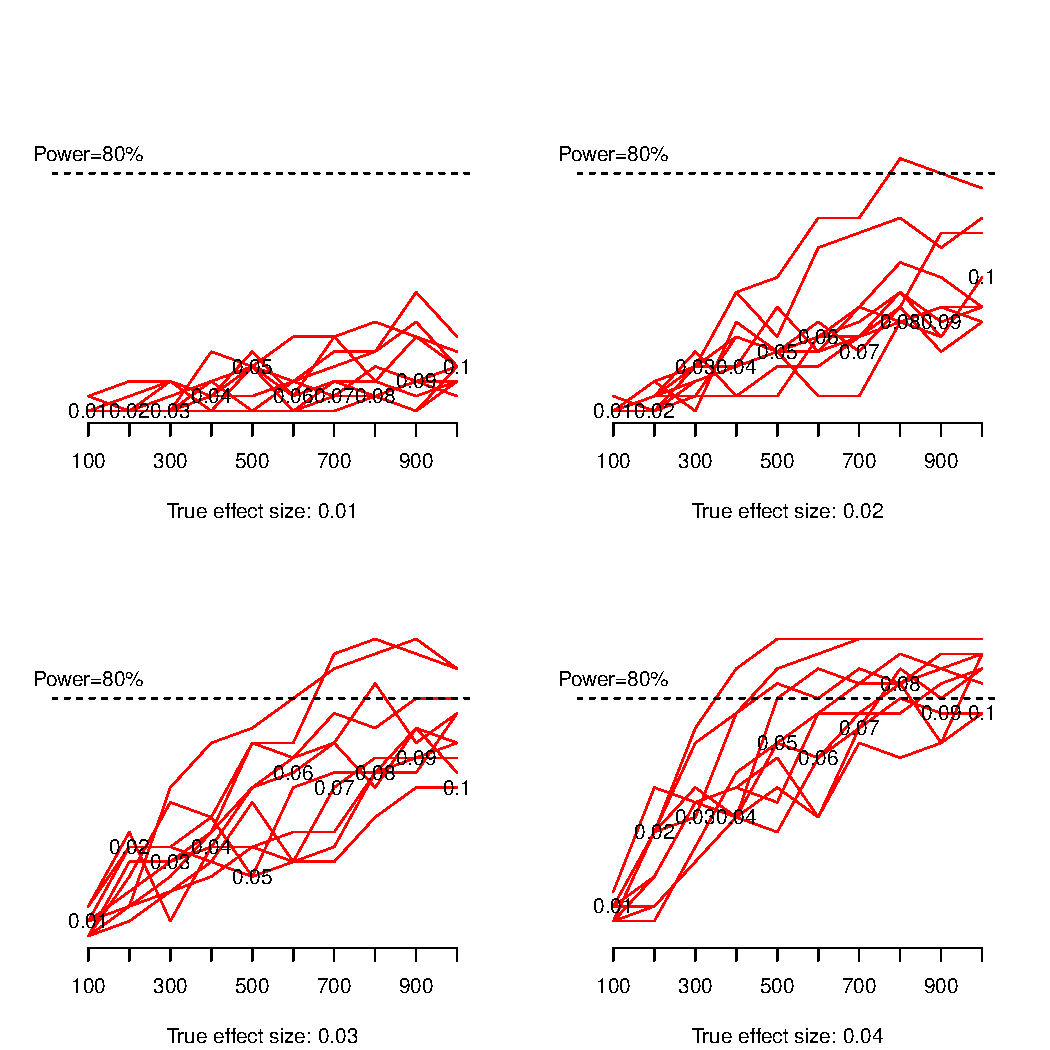
\includegraphics{Figures/unnamed-chunk-6-1.pdf}
\caption{Power simulations. Relationship between simulated statistical
power (y-axis) and group size (x-axis). Data are simulated from a
binomial model with varying probability of success for subjects in
treatment and control groups; Effect size is the difference in
probability of success between control and treatment groups which is
reported at the bottom of each picture; Next to each curve we have
reported the corresponding probability of success in the control group.
Significance computed using Chi-square test statistics with
\(\alpha=0.05\). We used 20 simulations for each instance.}
\end{figure}

\subsection{Context}\label{context}

We designed two interventions in collaboration with HeroX.com, a
crowdsourcing platform. We view HeroX as an example of a competitive
(platform users make submissions solving a given problem and the top
submissions are awarded a cash prize) and collaborative environment,
respectively.

\subsection{Data}\label{data}

\renewcommand\refname{References}
\bibliography{library.bib}

\end{document}